\subsection{Overview}

Our S\&C subsystem consists of :
\begin{itemize}
    \item Control Boards: 
    \begin{itemize}
            \item Braking Controller
            \item Thermal (Cooling) Controller
            \item Telemetry Controller
    \end{itemize}

    \item Telemetry Device: 
    \begin{itemize}
            \item CAN Bus
            \item Telemetry Transceiver
            \item Network Transceiver
            \item GUI/Logging system
    \end{itemize}
\end{itemize}
In this section, the main components of the sensor network and software architecture shall be described, as well as their basic functionality. A special focus shall be made on how safety mechanisms are implemented in these systems. Extensive design descriptions are expected for, if applicable:

\subsection{Control Boards}
\subsubsection{Introduction}
\begin{enumerate}
    \item Overview of all control boards (Brakes, Thermal, Telemetry):
    \begin{itemize}
        \item Brakes Controller: \\
        The brakes board controls the pod's friction braking system.
        It drives the solenoid valves that are connected to the braking mechanisms.
        The board's design engage the brakes by default for safety, releasing them only when all safety criteria are met,
        which come from the sensors and user commands. 
        It utilizes a Texas Instrument C2000 series microcontroller.
        \item Thermal (Cooling) Controller: The thermal board drives the coolant pump via a PWM to a MOSFET bridge, adjusting the pump speed based on the feedback from temperature and flowrate sensors in the cooling loop.
        The system design also includes continuous monitoring of temperatures at multiple (critical) areas of the Fermion to detect overheating. 
        \item Telemetry Controller: The telemetry board is the pod's communication system, facilitating bidirectional data exchange between the pod and the user device, typically a laptop.
        It is responsible for sending commands to the pod and receiving diagnostic and sensor information in return.
        The system uses the CAN bus for communication in the pod.
    \end{itemize}
  
Our Sense\&Control system includes three main boards:
For the Braking Managament System \textbf{TO BE ADDED}

The Thermal Management Controller is responsible for cooling the Traction Components, i.e., Motor and Traction Controller. The actuator is the coolant pump which is controlled  with the feedback of the temperature of coolant in the cooling loop (Refer to Diagram for Visualisation).  The Pump Speed is controlled via PWM to the MOSFET Bridge. The PWM duty cycle is simply calculated from a lookup table that is referenced to the temperature difference between target and actual temperatures. The only safety feature to be developed is to issue an emergency stop signal to HV Systems in the event the coolant temperature exceeds a critical temperature.
Finally, the Telemetry Unit is responsible for receiving commands from, and transmitting diagnostic and sensor information to the commanding PC. The Telemetry unit then receives and broadcasts information as well as commands on the CAN bus as a Master Controller to all the slave devices. 
    \item Diagram with the connection of all boards with NAP and control station:
    Für Ian: Das ist als Netzwerkdiagramm gedacht. Einfach telemetrysystems.png nehmen, ggf. kennzeichnen was unser NAP und control station ist. Das unten kommt erst später-

The implementation of the hardware architecture goes as follows FÜR IAN: habe hier aktuelle graphiken eingefügt, beschriftungen angepasst. musst du halt irgendwo an die richtige stelle schieben. schau mal was begin{figure}[h] macht.:
    \begin{figure}
        \centering
        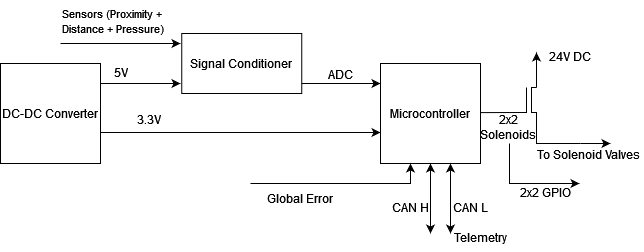
\includegraphics[width=\linewidth]{texfiles/elec/eimg/Brakesystems}
        \caption{Brakes Controller NAP Connections} 
        \label{fig:Brakes Controller NAP Connections}
    \end{figure}
 \begin{figure}
        \centering
        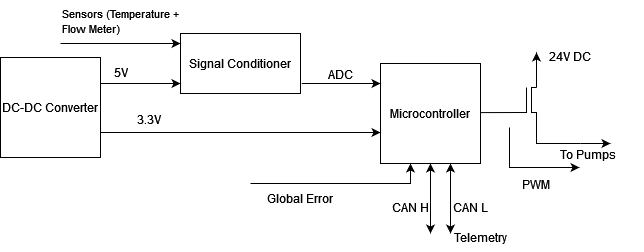
\includegraphics[width=\linewidth]{texfiles/elec/eimg/thermalsystems}
        \caption{Thermal Controller NAP Connections}
        \label{fig:Thermal Controller NAP Connections}
    \end{figure}
 \begin{figure}
        \centering
        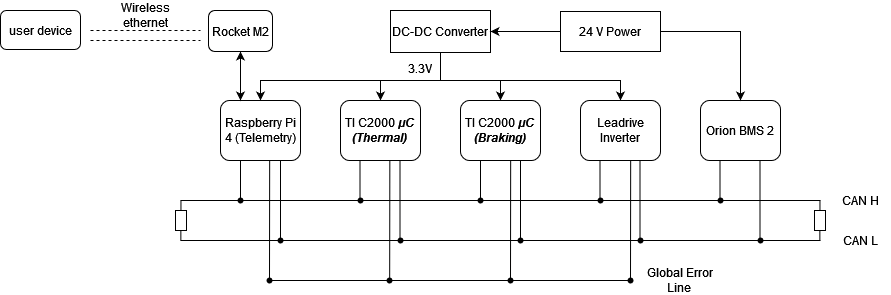
\includegraphics[width=\textwidth]{texfiles/elec/eimg/telemetrysystems}
        \caption{Telemetry Unit Hardware Architecture}
        \label{fig:Telemetry Unit Hardware Architecture}
    \end{figure}

    \item Communication protocols used: 
\begin{enumerate}
    \item Control Area Network (CAN): CAN was implemented as the inter-board communication protocol. This decision is inspired by the automotive industry, where CAN has been used for decades as a robust and physically reliable protocol.
    To add to that, many of our OEM devices (only) support CAN communication. Für IAN add Link to CAN Description online
    \item LAN: Used to transmit data between the Telemetry Unit and command PC.

    \item Serial Peripheral Interface (SPI): Synchronous, full-duplex communication protocol used for connecting peripheral devices.The master device generates the clock signal on SCLK while transmitting data to the slave device via MOSI, and the slave device responds with data on MISO. Communication occurs simultaneously in both directions, what allows high-speed data transfer between devices. \\
    Inter-Integrated Circuit (I2C): Multi-device communication protocol used for connecting sensors.
\end{enumerate}

\end{enumerate}

% Merged detailed content from the first snippet

\subsection{State Machine of the Vehicle}
% Continue with the structured format from the second snippet, ensuring to merge relevant content from the first snippet into these sections.

We use different states in each component. Our pod has the following states:
Generally (and in the main control of the pod), we have the following structure:

\subsection{Code Architecture and Class Diagram}
% Insert content from the first snippet related to Code Architecture here.
\subsubsection{Brakes Controller}
The software follow a simple state:
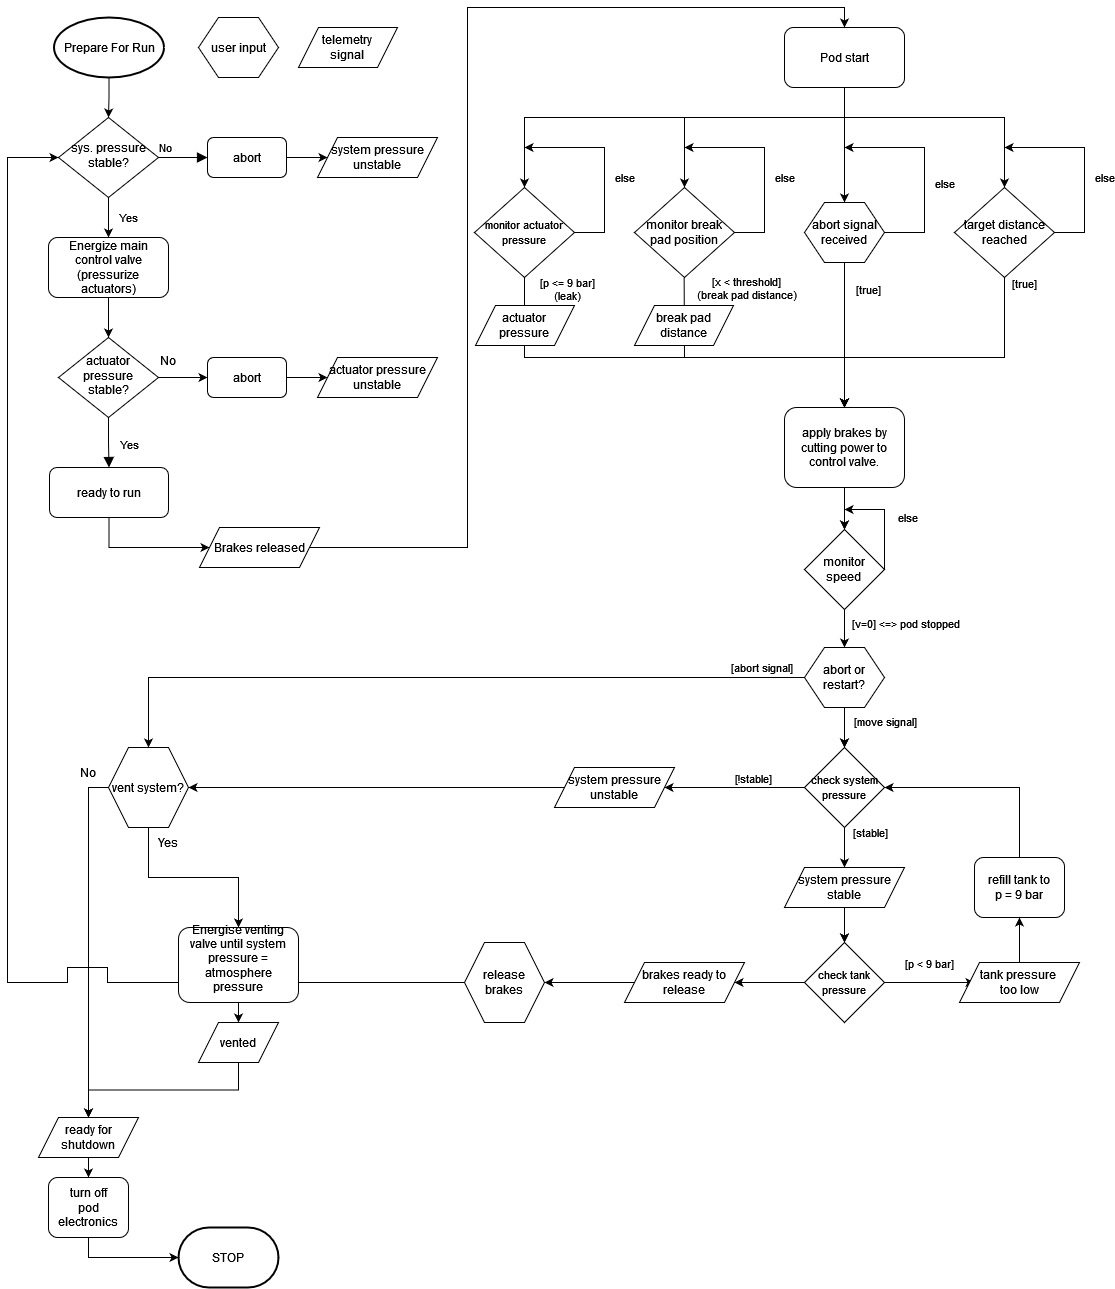
\includegraphics[width=\textwidth]{texfiles/elec/eimg/brakesoftware_ext}
\subsubsection{Thermal Controller}
Software goes along the following state diagram: \\
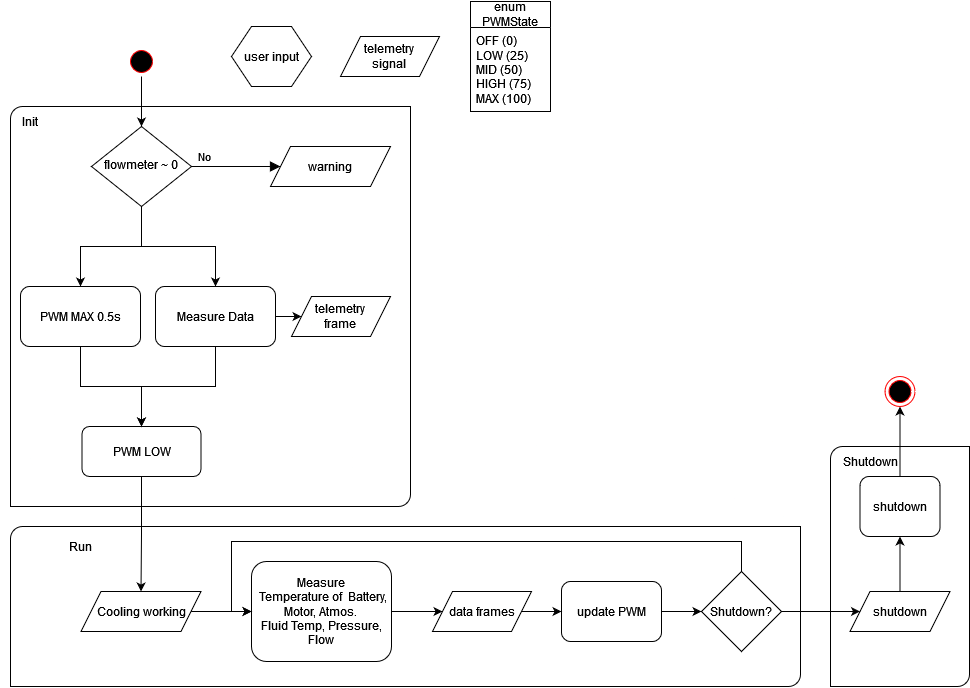
\includegraphics[width=\textwidth]{texfiles/elec/eimg/thermalsystemsflowchartsoftware}

The following hardware architecture is to be implemented:

\subsubsection{Telemetry Device}
The software adheres to this chart: \\
To Ian: Include the state machines at Software Rationale.
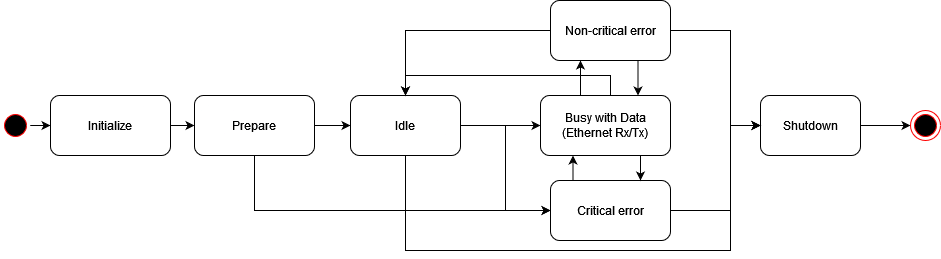
\includegraphics[width=\textwidth]{texfiles/elec/eimg/telemetrystate.png}

\subsection{Control Boards/Units in the Vehicle}
% Insert content from the first snippet related to Control Boards/Units in the Vehicle here.

\begin{enumerate}
    \item Brakes Controller
    \begin{enumerate}
        \item Requirements of the board.
        Parts List:
            \begin{table}[h]
                \centering
                \begin{adjustbox}{width=\textwidth,center}
                    \begin{tabular}{|c|c|c|c|c|c|c|}
                    \hline
                    \textbf{Amount} & \textbf{Name} & \textbf{Company (Serial Number)} & \textbf{Dimensions (mm x mm x mm)} & \textbf{Weight (kg)} & \textbf{Nominal Voltage} & \textbf{Expected max current} \\
                    \hline
                    38 & Additional Temperature Sensors (NTC, 10k Ohm) & Mouser & 1000 x 3 x 3 & $200 \times 10^{-6}$ & - & - \\
                    \hline
                    1 & Coolant Pump & Unknown & Unknown & Unknown & Unknown & Unknown \\
                    \hline
                    1 & MOSFET Bridge & Unknown & Unknown & Unknown & Unknown & Unknown \\
                    \hline
                    \end{tabular}
                \end{adjustbox}
                \caption{Description of Components}
                \label{tab:components}
            \end{table}
        \item Hardware Rationale (HW design and concerns). \\
        Critical points: Safety. The brakes should engage by default, and only release when all safety criteria are met. The board should be designed to be fail-safe, and process information and requests quickly.
        Our brakes controller's \href{https://drive.google.com/file/d/1a7zaJbmfFdLdrrGtLt2_ySVTqbc168NL/}{hardware design documentation} is uploaded (non-publicly) online, to view for the reader. We show only the schematic here. 
        \begin{figure}
            \centering
            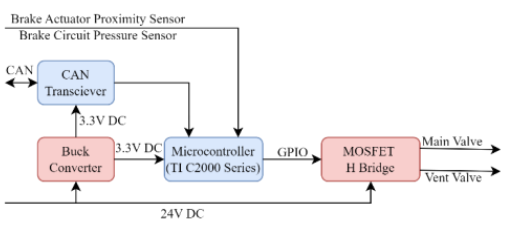
\includegraphics[width=\linewidth]{texfiles/elec/eimg/Brakes_architecture}
            \caption{Brakes Controller Hardware Schematic}
            \label{fig:Brakes Controller Hardware Schematic}
        \end{figure}


        \item Firmware Rationale (Internal State machine and design concerns).
        No stuck loops. Real-life transport scenario: Re-release of brakes is possible. 
        Für Ian zum ausformulieren.

        \item Testing and validation plan.


    \end{enumerate}

    \item Thermal Controller
        \begin{enumerate}
            \item Requirements of the board.\\
            Should drive the coolant pump. The control algorithm, planned as a PID controller, is to be implemented, but not necessary. We can let the thermal system run on a on-off scheme, which is less effective, but easier.

            \item Hardware Rationale (HW design and concerns).
            Simplicity. The brakes controller design was big. The thermal controller is mainly gathering sensor data, such as temperature sensors, and flow rate, and controlling the pump. The pump is a simple on-off device, and the temperature control is not critical. 
            \item Firmware Rationale (Internal State machine and design concerns).
            \item Testing and validation plan.
            \begin{itemize}
                \item Test maximum volume (mass transfer) power of pump.
                \item The temperature sensors should be tested for their accuracy and deviance.
                \item The control algorithm should be tested for its effectiveness, and delay due to mechanical and thermodynamical factors.
                \item Test flow system sensors for accuracy and deviance.
                \item Test maximum cooling power of pump. This testing scenario will not be used during the competition.
            \end{itemize}
        \end{enumerate}

        \item Telemetry Controller
        \begin{enumerate}
            \item Requirements of the board.
            Parts Lists
                \begin{table}[H]
                    \centering
                    \begin{tabular}{|l|l|l|}
                    \hline
                    \textbf{Part} & \textbf{Manufacturer} & \textbf{Description} \\ \hline
                    Raspberry Pi Zero 2 W & Raspberry & Microcontroller for telemetry \\ \hline
                    Raspberry Pi 4 B & Raspberry & Computer for telemetry \\ \hline
                    MC3479 & Memsic & 3-Axis Accelerometer \\ \hline
                    RS485 CAN HAT & Waveshare & CAN adapter for RPI4B \\ \hline
                    \end{tabular}
                    \caption{Telemetry System Parts List}
                    \label{tab:my-table}
                \end{table}
            \item Hardware Rationale (HW design and concerns).
            
            \item Firmware Rationale (Internal State machine and design concerns).

            \item Testing and validation plan.
        \end{enumerate}
\end{enumerate}

\subsection{Communication and Navigation}
\subsubsection*{Communication}
For communication, we use our telemetry system, transmitting bidirectionally telemetry data and commands to the pod. The telemetry system uses the CAN bus, which is a robust and reliable protocol which will not be explained further, presuming that the reader is already familiar with it. \\
The VCU, in this sense, is a Raspberry Pi 4B, which is connected to the CAN bus via a RS485 CAN HAT. 
Through its connectivity abilities, we can connect to a Wireless LAN system for (necessary) remote control. We use the Rocket M2 as a transmitter. A short estimation of scales of speed between electromagnetic fields and the speed of common ground transportation modes show that we have not reached the speed where the Doppler effect of the signals play any significant role, so we do not take that into consideration. We use the open-source GUI system of Swissloop and plan to develop our own data logging system as an addition. The addition we plan to add to the GUI system are the following:
\begin{itemize}
    \item (Cosmetic) adaption to the Fermion, including \begin{itemize}
        \item the battery pack layout for both batteries
        \item the thermal system data
        \item acceleration data
        \item check for abnormal situations, like \begin{itemize}
            \item 
        \end{itemize}
    \end{itemize}
    \item Time Counter since start of run
    \item More informative audiovisual feedback
\end{itemize} 

\subsubsection*{Navigation}
Our navigation system does not incorporate railway-like switches, nor GPS due to the track's short length. Instead, the pod solely uses an accelerometer and speed sensors to measure the velocities of both the front (guiding) wheel and the back (propulsion) wheel,
determining the pod's dynamics. This also includes vibrations.\\
In this iteration, we have clearly defined competition rules, and hence stick to simple acceleration/velocity/distance curveds. In the future, we plan to implement a more complex navigation system, including a system that can compute the acceleration/speed automatically, which is a more realistic use case.
\begin{enumerate}
    \item Design requirements
The Telemetry Devices possesses the following properties and constraints

\begin{table}[htbp]
    \centering
    \begin{tabular}{|l|l|}
        \toprule
        \textbf{Constraint/Specification} & \textbf{Value} \\
        \midrule
        Operating Voltage & 24 V \\
        Mass & $<200$ g \\
        Budget & $<500$ € \\
        Range & 0.2 Km LOS \\
        Communication Frequency & 2.4GHz \\
        \bottomrule
    \end{tabular}
     \caption{Specification of the Telemetry Unit Constraints}
\label{tab:Telemetry Constraints}
\end{table}

To allow the correct transmission of information, the following CAN signals should be sent by the Telemetry unit to all the Slave devices:
\begin{table}[htbp]
    \centering
    \begin{tabular}{|l|l|}
        \textbf{Device} & \textbf{Command} \\
        \midrule
        Traction Controller & Target Speed or Torque \\
        Battery Pack & Emergency Disconnect \\
        Thermal Management System & Target Temperature \\
        Brakes Controller & Brake Engage Command \\
        \bottomrule
    \end{tabular}
 \caption{Devices and their commands}
\label{tab:Command devices.}
\end{table}

\begin{table}[htbp]
    \centering
    \begin{tabular}{|l|l|}
        \toprule
        \textbf{Device} & \textbf{Signal} \\
        \midrule
        All & Emergency / Error Messages \\
        Traction Controller & Speed, Phase Currents, Inverter Module \& Motor Temperature \\
        Battery Pack & Pack Voltage, Pack Current, Cell Temperatures, SoC \\
        Thermal Systems & Temperatures \\
        \bottomrule
    \end{tabular}
    \caption{CAN signals received by the devices}
\label{tab:CAN signals.}
\end{table}

All the above signals shall be transmitted to the command PC over Wireless communication.

    \item Network Diagrams:
The overall system can be described with the following chart:
\begin{figure}
    \centering
    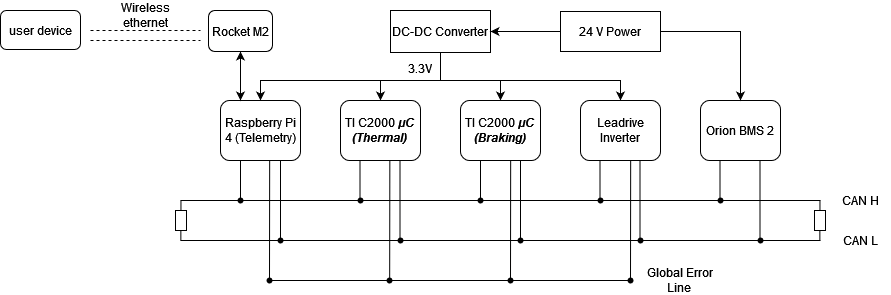
\includegraphics[width=\textwidth]{texfiles/elec/eimg/telemetrysystems.png}
    \caption{Overall Structure of the Telemetry Sytem}
    \label{fig:enter-label}
\end{figure}
%I dont think we have
    \item Sub-networks Diagrams (Track, Vehicle and Spectators)

    \item Graphical User Interface (GUI)
\end{enumerate}


% Insert content from the first snippet related to GUI here.

% Continue merging additional sections and sub-sections from the first snippet into the structured format of the second snippet as needed.

